% Paper 2: overview of how the study runs (tasks, checks, sessions, decision method, decision).
% Build: pdflatex paper2_study_overview.tex  (standalone, cropped, vector output)
% Designed at print size: 12.2 cm wide (LNCS text width). Style follows _style_reference_mesa.tex.
\documentclass[border=1pt]{standalone}
\usepackage[T1]{fontenc}
\usepackage{helvet}
\renewcommand{\familydefault}{\sfdefault}
\usepackage{calc}
\usepackage{tikz}
\usetikzlibrary{positioning,arrows.meta,calc}

% Same color roles as the reference figure
\definecolor{inF}{HTML}{F7F7F7}  \definecolor{inB}{HTML}{555555}  % inputs: gray
\definecolor{mpF}{HTML}{D5E5F7}  \definecolor{mpB}{HTML}{3A78C2}  % checks: blue
\definecolor{sAF}{HTML}{F7CD95}  \definecolor{sAB}{HTML}{C06F00}  % agent sessions: orange
\definecolor{sBF}{HTML}{A9D8B9}  \definecolor{sBB}{HTML}{2A7F4F}  % decision method: green
\definecolor{dcF}{HTML}{86C29D}  % decision: darker green fill, same green border
\definecolor{arr}{HTML}{333333}

% at 12.2 cm: columns of 3.50, 3.90 and 3.30 cm; gaps of 1.00 and 0.50 cm
\newlength{\wA}\setlength{\wA}{3.50cm}
\newlength{\wB}\setlength{\wB}{3.90cm}
\newlength{\wC}\setlength{\wC}{3.30cm}
\newlength{\gapA}\setlength{\gapA}{1.00cm}
\newlength{\gapB}\setlength{\gapB}{0.50cm}
\newlength{\hTop}\setlength{\hTop}{1.93cm}
\newlength{\hBot}\setlength{\hBot}{1.93cm}
\newlength{\rowgap}\setlength{\rowgap}{0.80cm}

\tikzset{
  box/.style={draw, line width=0.6pt, rounded corners=3pt, inner sep=0pt,
    inner xsep=4.5pt, anchor=north west},
  link/.style={-{Stealth[length=4.2pt,width=3.6pt]}, line width=0.75pt, draw=arr},
  lab/.style={font=\fontsize{7}{8.4}\selectfont, text=arr, inner sep=1.5pt, align=left},
}

% bullet list at 7 pt, same settings as the reference
\newenvironment{blist}{%
  \fontsize{7}{8.4}\selectfont\raggedright
  \begin{list}{\textbullet}{\setlength{\leftmargin}{6.5pt}\setlength{\labelsep}{2.8pt}%
      \setlength{\labelwidth}{3.7pt}\setlength{\itemsep}{0pt}\setlength{\parsep}{0pt}%
      \setlength{\topsep}{0pt}\setlength{\partopsep}{0pt}\raggedright}}%
  {\end{list}}

% box content: #1 box width, #2 box height, #3 title, #4 body; top aligned
\newcommand{\boxcontent}[4]{%
  \parbox[c][#2][t]{#1-9pt}{%
  \vspace*{4.5pt}%
  {\centering\fontsize{8}{9.6}\selectfont\bfseries #3\par}%
  \vspace{2.5pt}%
  #4}}

\begin{document}
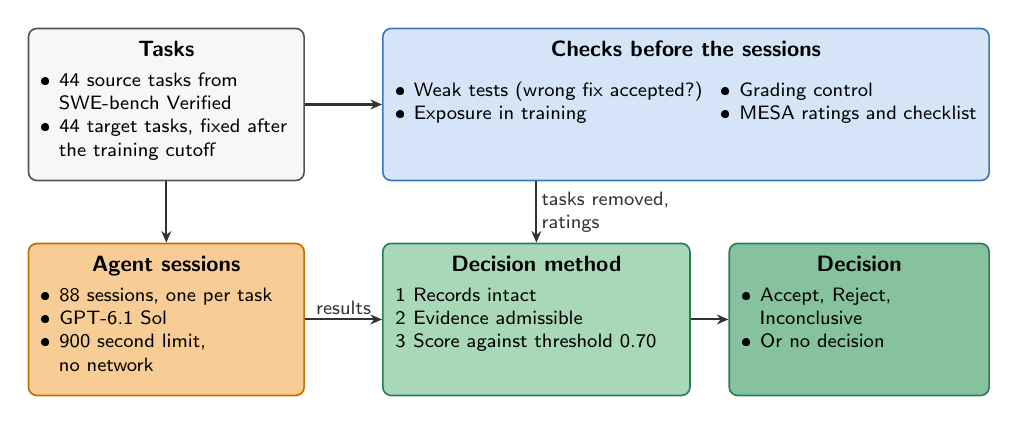
\begin{tikzpicture}
  \pgfmathsetlengthmacro{\xA}{0pt}
  \pgfmathsetlengthmacro{\xB}{\wA+\gapA}
  \pgfmathsetlengthmacro{\xC}{\wA+\gapA+\wB+\gapB}
  \pgfmathsetlengthmacro{\yBot}{-\hTop-\rowgap}

  % top row: tasks and the checks before the sessions
  \node[box, fill=inF, draw=inB] (T) at (\xA,0)
    {\boxcontent{\wA}{\hTop}{Tasks}{\begin{blist}
      \item 44 source tasks from \mbox{SWE-bench} Verified
      \item 44 target tasks, fixed after the training cutoff
    \end{blist}}};
  \node[box, fill=mpF, draw=mpB] (K) at (\xB,0)
    {\boxcontent{\wB+\gapB+\wC}{\hTop}{Checks before the sessions}{%
      \begin{minipage}[t]{0.56\linewidth}\begin{blist}
        \item Weak tests (wrong fix accepted?)
        \item Exposure in training
      \end{blist}\end{minipage}%
      \begin{minipage}[t]{0.44\linewidth}\begin{blist}
        \item Grading control
        \item MESA ratings and checklist
      \end{blist}\end{minipage}}};

  % bottom row: sessions, decision method, decision
  \node[box, fill=sAF, draw=sAB] (S) at (\xA,\yBot)
    {\boxcontent{\wA}{\hBot}{Agent sessions}{\begin{blist}
      \item 88 sessions, one per task
      \item GPT-6.1 Sol
      \item 900 second limit, no~network
    \end{blist}}};
  \node[box, fill=sBF, draw=sBB] (M) at (\xB,\yBot)
    {\boxcontent{\wB}{\hBot}{Decision method}{\begin{blist}
      \item[1] Records intact
      \item[2] Evidence admissible
      \item[3] Score against threshold 0.70
    \end{blist}}};
  \node[box, fill=dcF, draw=sBB] (D) at (\xC,\yBot)
    {\boxcontent{\wC}{\hBot}{Decision}{\begin{blist}
      \item Accept, Reject, Inconclusive
      \item Or no decision
    \end{blist}}};

  % arrows: straight, none cross
  \draw[link] (T.east) -- (K.west);
  \draw[link] (T.south) -- (S.north);
  \draw[link] (S.east) -- node[lab, above] {results} (M.west);
  \draw[link] (K.south -| M.north) -- node[lab, right] {tasks removed,\\ ratings} (M.north);
  \draw[link] (M.east) -- (D.west);
\end{tikzpicture}
\end{document}
